\documentclass[11pt]{article}
\usepackage[margin=1in]{geometry}
\usepackage[utf8]{inputenc}
\usepackage[T1]{fontenc}
\usepackage{amsmath,amssymb}
\usepackage{booktabs}
\usepackage{enumitem}
\usepackage{tikz}
\usetikzlibrary{arrows.meta,positioning}
\usepackage[hidelinks]{hyperref}

\newcommand{\ARSnode}[1]{%
  \node[circle,draw,minimum size=7mm,inner sep=0pt] (#1) {$#1$};%
}
\newcommand{\ARSnodeat}[2]{%
  \node[circle,draw,minimum size=7mm,inner sep=0pt, #2] (#1) {$#1$};%
}
\tikzset{>={Stealth[length=3mm]}, every loop/.style={looseness=7}}

\title{CPSC 354 — Report}
\author{Ray Hettleman \quad \texttt{rhettleman@chapman.edu}}
\date{\today}

\begin{document}
\maketitle
\tableofcontents

% =========================================================
\section{Assignment 1: MIU System — Can we derive \texttt{MIII} from \texttt{MI}?}

\subsection*{Problem (restated)}
Starting from \texttt{MI}, and using the MIU rules:
\begin{enumerate}[label=\Roman*.]
  \item If a string ends with \texttt{I}, you may append \texttt{U}.
  \item From \texttt{Mx} you may infer \texttt{Mxx}.
  \item Replace any occurrence of \texttt{III} by \texttt{U}.
  \item Delete any occurrence of \texttt{UU}.
\end{enumerate}
Determine whether \texttt{MIII} is derivable. Explain your reasoning.

\subsection*{Solution}
\textbf{Idea.} Track the count of \texttt{I}'s. Rule~I and Rule~IV do not change that count. Rule~II doubles it; Rule~III removes 3 but can only apply if 3 consecutive \texttt{I}'s already exist.

Starting from \texttt{MI} (one \texttt{I}), the only growth is doubling. So after the first step the number of \texttt{I}'s is always even. Removing triples never gives exactly three. So \texttt{MIII} cannot appear.

\subsection*{Conclusion}
It is \textbf{impossible} to derive \texttt{MIII} from \texttt{MI}.  
Reason: the number of \texttt{I}'s is never equal to three under these rules.

% =========================================================
\section{Assignment 2: ARS Pictures \& Properties}

\subsection*{Task (restated)}
For each given abstract reduction system (ARS) $(A,R)$: draw the graph, decide
whether it is terminating, confluent, and whether it has unique normal forms (UNFs).

\subsection*{Instances}

\paragraph{1.\; $A=\varnothing$}
No nodes/edges. \emph{Terminating:} True. \emph{Confluent:} True. \emph{UNFs:} True.

\paragraph{2.\; $A=\{a\},\; R=\varnothing$}
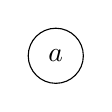
\begin{tikzpicture}
  \ARSnode{a};
\end{tikzpicture}

Normal forms: $a$. Terminating: True. Confluent: True. UNFs: True.

\paragraph{3.\; $A=\{a\},\; R=\{(a,a)\}$}
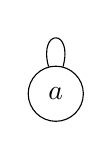
\begin{tikzpicture}
  \ARSnode{a};
  \path (a) edge[loop above] (a);
\end{tikzpicture}

Infinite $a\to a\to\cdots$: Terminating: \textbf{False}. Confluent: \textbf{True}. UNFs: \textbf{False}.

\paragraph{4.\; $A=\{a,b,c\},\; R=\{(a,b),(a,c)\}$}
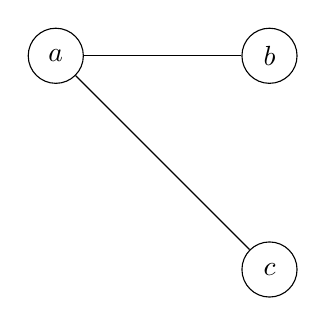
\begin{tikzpicture}[node distance=20mm]
  \ARSnode{a};
  \ARSnodeat{b}{right=of a}
  \ARSnodeat{c}{below=of b}
  \draw (a) edge (b) (a) edge (c);
\end{tikzpicture}

$b,c$ are normal; from $a$ two distinct NFs. Terminating: \textbf{True}. Confluent: \textbf{False}. UNFs: \textbf{False}.

\paragraph{5.\; $A=\{a,b\},\; R=\{(a,a),(a,b)\}$}
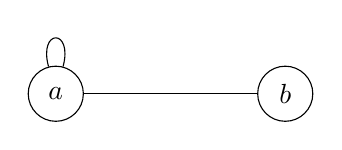
\begin{tikzpicture}[node distance=22mm]
  \ARSnode{a};
  \ARSnodeat{b}{right=of a}
  \draw (a) edge[loop above] (a) (a) edge (b);
\end{tikzpicture}

$b$ is normal; every element has the (unique) NF $b$. Terminating: \textbf{False}. Confluent: \textbf{True}. UNFs: \textbf{True}.

\paragraph{6.\; $A=\{a,b,c\},\; R=\{(a,b),(b,b),(a,c)\}$}
\begin{tikzpicture}[node distance=22mm]
  \ARSnode{a};
  \ARSnodeat{b}{right=of a}
  \ARSnodeat{c}{below=of b}
  \draw (a) edge (b) (a) edge (c) (b) edge[loop above] (b);
\end{tikzpicture}

Non-terminating via $b\to b$; $c$ is normal, $b$ has no NF.
Confluent: \textbf{False}. Terminating: \textbf{False}. UNFs: \textbf{False}.

\paragraph{7.\; $A=\{a,b,c\},\; R=\{(a,b),(b,b),(a,c),(c,c)\}$}
\begin{tikzpicture}[node distance=22mm]
  \ARSnode{a};
  \ARSnodeat{b}{right=of a}
  \ARSnodeat{c}{below=of b}
  \draw (a) edge (b) (a) edge (c) (b) edge[loop above] (b) (c) edge[loop right] (c);
\end{tikzpicture}

Both $b$ and $c$ loop; no NFs reachable from $a$. Terminating: \textbf{False}. Confluent: \textbf{False}. UNFs: \textbf{False}.

\subsection*{Summary Table}
\begin{tabular}{@{}clccc@{}}
\toprule
\# & $(A,R)$ & confluent & terminating & unique normal forms \\
\midrule
1 & $(\varnothing,\varnothing)$ & True & True & True \\
2 & $(\{a\},\varnothing)$ & True & True & True \\
3 & $(\{a\},\{(a,a)\})$ & True & False & False \\
4 & $(\{a,b,c\},\{(a,b),(a,c)\})$ & False & True & False \\
5 & $(\{a,b\},\{(a,a),(a,b)\})$ & True & False & True \\
6 & $(\{a,b,c\},\{(a,b),(b,b),(a,c)\})$ & False & False & False \\
7 & $(\{a,b,c\},\{(a,b),(b,b),(a,c),(c,c)\})$ & False & False & False \\
\bottomrule
\end{tabular}

\subsection*{All 8 combinations}
\begin{tabular}{@{}ccccl@{}}
\toprule
confluent & terminating & unique NFs & example \\
\midrule
True  & True  & True  & e.g.\ ARS 2 (or 1) \\
True  & True  & False & \textit{Impossible} \\
True  & False & True  & ARS 5 \\
True  & False & False & ARS 3 \\
False & True  & True  & \textit{Impossible} \\
False & True  & False & ARS 4 \\
False & False & True  & \textit{Impossible} \\
False & False & False & ARS 6 (or 7) \\
\bottomrule
\end{tabular}

% =========================================================
\section{Assignment 3: Exercises 5 and 5b}

\subsection*{Problem (restated)}
Exercise 5 asks us to analyse a given ARS and check for termination, confluence,
and unique normal forms.  
Exercise 5b asks us to consider a small variation and explain the difference.

\subsection*{Solution to Exercise 5}
For the ARS with $A=\{a,b\}$ and rules $a\to a$, $a\to b$:
\begin{itemize}
  \item There is a loop $a\to a$, so the system is \textbf{not terminating}.
  \item From $a$ we can still reach $b$, and $b$ is normal. Every path from $a$
    eventually has the option to reach $b$, and once at $b$ no rules apply.
  \item Thus the ARS is \textbf{confluent}: all reductions can be joined at $b$.
  \item Normal forms are unique: everything reduces to $b$.
\end{itemize}

\subsection*{Solution to Exercise 5b}
Now suppose we add $c$ with $a\to c$ and $c\to c$:
\begin{itemize}
  \item Again, $a$ can reduce to both $b$ and $c$.
  \item But $c$ loops forever and never reaches $b$.
  \item That means the system is no longer confluent: starting from $a$ you can end
    in either the normal form $b$ or the non-terminating loop on $c$.
  \item Unique normal forms are therefore lost.
\end{itemize}

\subsection*{Conclusion}
Exercise 5 shows a non-terminating but confluent system (everything has the unique NF $b$).  
Exercise 5b shows that adding another looping branch breaks confluence, since from $a$
different outcomes are possible.

% =========================================================
\section{Assignment 4: Termination}

\subsection{HW 4.1}
Consider the following algorithm:
\begin{verbatim}
while b != 0:
    temp = b
    b = a mod b
    a = temp
return a
\end{verbatim}

\paragraph{Conditions.} Termination is guaranteed if $a, b$ are nonnegative integers and $b > 0$ initially.

\paragraph{Measure function.} Define $\varphi(a,b) = b$.  
At each step $b$ is replaced by $a \bmod b$, which is strictly smaller than $b$ but always nonnegative. Therefore $\varphi$ decreases with every iteration.

\paragraph{Conclusion.} Since $\varphi(a,b)$ is a nonnegative integer that strictly decreases, the loop must terminate. The algorithm is in fact Euclid’s algorithm for $\gcd(a,b)$.

\subsection{HW 4.2}
Consider the following fragment of an implementation of merge sort:
\begin{verbatim}
function merge_sort(arr, left, right):
    if left >= right:
        return
    mid = (left + right) / 2
    merge_sort(arr, left, mid)
    merge_sort(arr, mid+1, right)
    merge(arr, left, mid, right)
\end{verbatim}

\paragraph{Measure function.} Define $\varphi(left,right) = right - left + 1$, the length of the current subarray.

\paragraph{Proof.} Each recursive call works on a subarray that is strictly smaller than the current one:
\begin{itemize}
  \item Initially, $\varphi(left,right) = n$ (array length).
  \item The recursive calls split the array into halves, so each subproblem has measure about $n/2$, strictly less than $n$.
  \item The base case $left \geq right$ gives $\varphi(left,right) \leq 1$, so recursion stops.
\end{itemize}

\paragraph{Conclusion.} Because the measure is a nonnegative integer that strictly decreases with each recursive call, \texttt{merge\_sort} always terminates.

\end{document}
